\documentclass[pmlr]{jmlr}% Proceedings of Machine Learning Research

\usepackage{booktabs}
\DeclareMathOperator*{\argmin}{arg\,min}

\jmlrvolume{319}
\jmlryear{2026}
\jmlrworkshop{IndabaX Nigeria 2026: Building Scalable AI That Works: From Research to Deployment in Resource-Constrained Environments}

\title[FedFairGNN]{FedFairGNN: A Privacy-Preserving and Fairness-Aware\titlebreak Federated Graph Neural Network for Fraud Detection}

\author{\Name{Quang-Vinh Dang} \Email{vinh.dq4@buv.edu.vn}\\
\addr School of Computing and Innovative Technologies\\
British University Vietnam\\
Hung Yen, Vietnam
\AND
\Name{Ngoc-Son-An Nguyen} \Email{annns25871@pgr.iuh.edu.vn}\\
\addr Faculty of Information Technology\\
Industrial University of Ho Chi Minh City\\
Ho Chi Minh City, Vietnam
}

\editor{Sakinat Folorunso, Roseline Ogundokun, and Francisca Oladipo}

\begin{document}

\firstpageno{74}

\maketitle

\begin{abstract}
Graph Neural Networks (GNNs) have emerged as a powerful tool for fraud detection. However, existing approaches often rely on centralized training, which raises privacy concerns when data is distributed across different institutions (e.g., banks). Federated Learning (FL) addresses this by enabling collaborative training without sharing raw data. Yet, FL on graph data faces unique challenges: (1) Graph heterogeneity across clients, and (2) Propagation of algorithmic bias. In this paper, we propose FedFairGNN, a novel framework that simultaneously ensures privacy, fairness, and utility. We introduce three key components: (1) \textbf{Fairness-Sensitive Edge Reweighting (FSER)} to mitigate structural bias in the graph, (2) \textbf{Fairness-Task Gradient Decomposition (FTGD)} with Differential Privacy to protect sensitive gradient information, and (3) \textbf{Bi-Objective Frank-Wolfe Aggregation (BFWA)} to optimize the global model under explicit fairness constraints. Extensive experiments simulating a federated network with $K=3$ clients on three real-world datasets (YelpChi, Amazon, Elliptic) demonstrate that FedFairGNN achieves a highly competitive performance-fairness trade-off while significantly reducing demographic disparity compared to existing baselines.
\end{abstract}

\begin{keywords}
Federated Learning, Graph Neural Networks, Fairness, Privacy, Fraud Detection.
\end{keywords}

\section{Introduction}
\label{sec:intro}

Financial fraud detection is a critical application of machine learning, preventing billions of dollars in losses annually. Graph Neural Networks (GNNs) have become the de facto standard for this task due to their ability to model complex relational patterns between users, transactions, and devices. However, traditional GNN approaches require centralized data storage, which violates modern privacy regulations (e.g., GDPR, CCPA) and raises security concerns for financial institutions.

Federated Learning (FL) offers a promising solution by allowing multiple clients (e.g., different banks) to collaboratively train a model without sharing their raw data. While FL privacy is a significant step forward, it introduces new challenges. First, graph data is notoriously non-IID (Independent and Identically Distributed), leading to performance degradation in standard FL aggregation. Second, and crucially, automated fraud detection systems are prone to algorithmic bias, often discriminating against certain demographic groups. In a federated setting, mitigating this bias is harder because the server does not have access to the data to measure or correct fairness directly.

In this paper, we present FedFairGNN, a unified framework that addresses the trilemma of Utility, Privacy, and Fairness in federated graph learning. Our contributions are:
\begin{enumerate}
  \item We propose a \textbf{Fairness-Sensitive Edge Reweighting (FSER)} mechanism that operates locally at each client to neutralize structural bias in the graph.
  \item We design a \textbf{Fairness-Task Gradient Decomposition (FTGD)} strategy that separates fairness-critical gradients from task gradients, applying Differential Privacy (DP) selectively to the former to preserve utility.
  \item We implement a \textbf{Bi-Objective Frank-Wolfe Aggregation (BFWA)} algorithm at the server, which optimizes the global model to satisfy strict fairness budgets without accessing local data.
\end{enumerate}

The remainder of this paper is organized as follows. Section~\ref{sec:related} reviews related work in graph-based fraud detection and federated learning. Section~\ref{sec:method} details the proposed FedFairGNN framework, including the mathematical formulation of FSER, FTGD, and BFWA. Section~\ref{sec:experiments} presents the experimental setup and discusses the results on three real-world datasets. Finally, Section~\ref{sec:conclusion} concludes the paper and outlines future directions.

\section{Related Work}
\label{sec:related}

\paragraph{GNN-based Financial Fraud Detection.} Graph Neural Networks have emerged as the dominant paradigm for financial fraud detection owing to their capacity to model relational patterns in transaction graphs \citep{cheng2025gnnfrauds}. Cheng et al. provide a comprehensive survey of GNN methodologies applied to financial fraud, identifying three key design challenges: camouflage resistance, class imbalance, and graph heterogeneity \citep{cheng2025gnnfrauds}. Addressing these challenges, Lou et al. propose the Context-Aware Fraud Detector (CAFD), which encodes temporal frequency and out-degree information alongside a random-dropping aggregator to suppress camouflaged fraudulent behaviour in transaction graphs \citep{lou2025cafd}. Although these works advance detection accuracy, they operate under centralised data assumptions and do not address demographic bias in model predictions, motivating the present work.

\paragraph{Federated Graph Learning and Anomaly Detection.} Collaborative fraud detection across financial institutions requires federated graph learning frameworks that operate without sharing raw transaction data. Wu et al. propose LG-FGAD, a federated graph anomaly detection framework that combines local-global awareness with dual knowledge distillation to preserve client personalisation while improving discriminative power \citep{wu2024lgfgad}. Deng et al. introduce a federated GNN for fake-review fraud detection in which differential privacy is applied to gradient updates shared between clients, demonstrating that combining privacy mechanisms with federated GNNs is feasible for real-world fraud scenarios \citep{deng2025dpfedgraph}. These works establish key building blocks for FedFairGNN, yet neither considers fairness constraints on protected demographic groups during federated aggregation.

\paragraph{Fairness in Graph Neural Networks.} Graph message-passing mechanisms propagate and amplify structural biases from the underlying graph topology, making fairness a first-class concern in GNN design \citep{lee2025dabgnn}. Zhu et al. propose FairINV, a graph fairness framework grounded in invariant learning that eliminates spurious correlations between sensitive attributes and node labels for multiple sensitive attributes within a single training session \citep{zhu2024fairinv}. Lee et al. present DAB-GNN, which disentangles, amplifies, and debiases node representations by learning separate sensitive and task-relevant encoders, achieving state-of-the-art fairness on benchmark datasets \citep{lee2025dabgnn}. Wo et al. address bias stemming from sensitive-attribute information in message passing through counterfactual data augmentation, showing that neighbourhood augmentation with contrasting sensitive attributes reduces demographic disparity without sacrificing classification accuracy \citep{wo2025counterfactual}. Collectively, these in-processing approaches for fair GNNs inform the design of our Fairness-Sensitive Edge Reweighting (FSER) module, which suppresses attention on cross-group edges exhibiting high embedding similarity rather than requiring adversarial training or graph augmentation.

\paragraph{Fair Graph Federated Learning.} Bridging fairness and federated graph learning is an emerging but nascent research direction. Pan et al. present the first incentive mechanism for fair graph federated learning, introducing gradient alignment and graph diversity criteria to quantify agent contributions and strike a balance between model accuracy and payoff fairness across participating institutions \citep{pan2024incentivefairgraphfl}. Notably, however, this work adopts a game-theoretic notion of fairness (contributor equity) rather than the demographic parity constraint on protected groups that is central to FedFairGNN. Li et al. propose a fairness-aware federated learning framework targeting heterogeneous data distributions across clients, incorporating a fairness penalty into local objectives and an adaptive aggregation scheme at the server \citep{li2024fairhetero}. Our Bi-Objective Frank-Wolfe Aggregation (BFWA) extends this line of work by casting server-side aggregation as a constrained optimisation problem on the probability simplex, with a hard upper bound on global Demographic Parity Difference rather than a soft regularisation penalty.

\paragraph{Fairness and Privacy in Federated Learning.} Enforcing fairness and privacy simultaneously in federated learning is fundamentally challenging because the two objectives often conflict: privacy mechanisms that mask sensitive attributes limit the ability to verify and correct demographic disparities. Chen et al. provide a comprehensive ACM Computing Surveys analysis of this trade-off, formalising the tension between differential privacy budget and the strength of fairness guarantees achievable in federated settings \citep{chen2024privacyfairness}. Rafi et al. survey fairness and privacy-preserving techniques across federated learning settings, cataloguing constraint-based, regularisation-based, and representation-learning approaches alongside their privacy-utility-fairness trade-offs \citep{rafi2024fairprivacysurvey}. Ling et al. propose FedFDP, which directly unifies fairness regularisation and differential privacy in a single federated objective, demonstrating that targeted noise calibration can preserve fairness improvement while satisfying formal $(\epsilon,\delta)$-DP guarantees \citep{ling2024fedfdp}. Our Fairness-Task Gradient Decomposition (FTGD) module advances beyond FedFDP by orthogonally decomposing the gradient into task and fairness subspaces and applying Gaussian DP noise exclusively to the fairness subspace, thereby preserving the full fraud-detection signal that would otherwise be degraded by uniform gradient perturbation.

\paragraph{Foundational Methods.} FedFairGNN builds on three recent technical foundations. Li et al. propose FedCompass \citep{li2024fedcompass}, an efficient cross-silo federated learning algorithm that employs a computing power-aware scheduler to synchronise client updates and reduce model staleness under heterogeneous data distributions; the group-aggregation communication protocol and weighted averaging paradigm established by FedCompass form the backbone that BFWA refines with fairness constraints on the probability simplex. Sha et al. introduce a heterogeneous graph neural network equipped with a graph attention mechanism that dynamically assigns relation-specific weights to transaction edges for credit-card fraud detection \citep{sha2025hetgat}; this attention-based, relation-aware message-passing design constitutes the base aggregation backbone that FSER extends with fairness-sensitive edge correction. Fu et al. provide a systematic review of differentially private federated learning \citep{fu2024dpflsurvey}, cataloguing central and local DP mechanisms, Gaussian noise calibration strategies, and privacy accounting methods that directly underpin the formal $(\epsilon,\delta)$-DP guarantee delivered by FTGD's targeted noise injection into the fairness gradient subspace.

\section{Our Method}
\label{sec:method}

\subsection{Problem Formulation}
Consider a federated graph learning setting with $K$ clients. Each client $k \in [K]$ holds a local graph $\mathcal{G}_k = (\mathcal{V}_k, \mathcal{E}_k, \mathbf{X}_k)$, where $\mathcal{V}_k$ is the set of nodes, $\mathcal{E}_k$ is the set of edges, and $\mathbf{X}_k \in \mathbb{R}^{|\mathcal{V}_k| \times d}$ is the feature matrix. Each node $v_i \in \mathcal{V}_k$ has a label $y_i \in \{0,1\}$ (0 for legitimate, 1 for fraud) and a sensitive attribute $s_i \in \{0,1\}$.

The goal is to collaboratively train a GNN model $f_\theta$ to minimize the global loss function $\mathcal{L}(\theta)$ while satisfying a global fairness constraint and preserving differential privacy. We define the fairness metric as the Demographic Parity Difference (DPD):
\begin{equation}
\Delta_{DP} = |P(\hat{y}=1 \mid s=0) - P(\hat{y}=1 \mid s=1)| \le \tau
\label{eq:dpd}
\end{equation}
where $\tau$ is a pre-defined fairness budget.

\subsection{Fairness-Sensitive Edge Reweighting (FSER)}
Graph homophily often leads to biased information propagation. FSER aims to mitigate this by reweighting edges during the aggregation phase. We adopt a Graph Attention Network (GAT) backbone. The standard attention coefficient $e_{ij}$ between node $i$ and neighbor $j$ is computed as:
\begin{equation}
e_{ij} = \text{LeakyReLU}(\mathbf{a}^\top[\mathbf{W}x_i \| \mathbf{W}x_j])
\label{eq:gat_attn}
\end{equation}
To incorporate fairness, we define a Fairness Risk Score $\phi_{ij}$ that penalizes edges between nodes with different sensitive attributes if their feature embeddings are highly similar (indicating potential confounding):
\begin{equation}
\phi_{ij} = \mathbb{I}(s_i \ne s_j) \cdot \text{ReLU}(\cos(x_i, x_j))
\label{eq:fser_risk}
\end{equation}
The reweighted attention coefficients are then:
\begin{equation}
\alpha_{ij} = \frac{\exp(e_{ij} - \beta \phi_{ij})}{\sum_{k \in \mathcal{N}_i} \exp(e_{ik} - \beta \phi_{ik})}
\label{eq:fser_attn}
\end{equation}
where $\beta$ is a hyperparameter controlling the strength of the fairness penalty. This mechanism effectively down-weights edges that are likely to propagate biased information.

\subsection{Fairness-Task Gradient Decomposition (FTGD)}
Standard Differential Privacy (DP) adds noise to the entire gradient, often degrading utility. We propose FTGD to decouple task-specific information from fairness-sensitive information. Let $\nabla \mathcal{L}_{task}$ be the gradient of the utility loss (e.g., BCE) and $\nabla \mathcal{L}_{fair}$ be the gradient of the local fairness regularization term.

We decompose the total gradient $g = \nabla \mathcal{L}_{task} + \lambda \nabla \mathcal{L}_{fair}$ into two orthogonal components:
\begin{align}
g_{fair} &= \nabla \mathcal{L}_{fair} \label{eq:gfair}\\
g_{task}^{\perp} &= g - \text{proj}_{g_{fair}}(g) = g - \frac{\langle g, g_{fair}\rangle}{\|g_{fair}\|^2} g_{fair} \label{eq:gtaskperp}
\end{align}
The decomposition assumes that the fairness and task gradients are meaningfully separable. In practice, this is empirically validated by measuring their low cosine similarity throughout training, indicating minimal overlap in their information-theoretic subspaces. Since sensitive information is primarily concentrated in $g_{fair}$, we apply Gaussian noise only to this component:
\begin{equation}
\tilde{g}_{fair} = \text{Clip}(g_{fair}, C) + \mathcal{N}(0, \sigma^2 I)
\label{eq:ftgd_noise}
\end{equation}
where $C$ is the clipping threshold and $\sigma$ is calibrated to satisfy $(\epsilon,\delta)$-DP. The final update sent to the server is $g_{update} = g_{task}^{\perp} + \tilde{g}_{fair}$. This preserves the utility-critical direction $g_{task}^{\perp}$ without noise.

\paragraph{Privacy Accounting and Utility Preservation.}
The privacy loss across multiple federated communication rounds is tracked using the Moments Accountant technique. By isolating the fairness-sensitive gradient $g_{fair}$ and applying noise strictly to its subspace, the effective dimension of the privatized vector is drastically reduced. This targeted noise injection prevents the catastrophic utility degradation typically observed when high-dimensional task gradients are corrupted by uniform isotropic DP noise. Furthermore, the clipping threshold $C$ is dynamically adapted using the median gradient norm of the historical updates, reducing the bias introduced by static clipping.

\subsection{Bi-Objective Frank-Wolfe Aggregation (BFWA)}
The server aggregates client updates to maximize utility subject to the global fairness constraint. This is formulated as a constrained optimization problem:
\begin{align}
\min_{w} \quad & \sum_{k=1}^{K} w_k \mathcal{L}_k(\theta) \label{eq:bfwa_obj}\\
\text{s.t.} \quad & \sum_{k=1}^{K} w_k \Delta_{DP,k}(\theta) \le \tau, \quad \sum_{k=1}^K w_k = 1, \quad w_k \ge 0 \label{eq:bfwa_constraint}
\end{align}
To solve this efficiently, we employ the Frank-Wolfe algorithm. We define the Lagrangian $L(w,\mu) = f(w) + \mu(g(w) - \tau)$. At each round $t$, we compute the gradient $\nabla_w L$ and find the linear minimization oracle (LMO) solution $s_t$:
\begin{equation}
s_t = \argmin_{s \in \Delta_K} \langle \nabla_w L(w_t,\mu_t), s\rangle
\label{eq:lmo}
\end{equation}
The weights are updated via $w_{t+1} = (1-\gamma_t)w_t + \gamma_t s_t$, and the dual variable $\mu$ is updated via gradient ascent:
\begin{equation}
\mu_{t+1} = \max\left(0, \mu_t + \eta_\mu\left(\sum_k w_{k,t}\Delta_{DP,k} - \tau\right)\right)
\label{eq:bfwa_dual}
\end{equation}
This allows the server to dynamically upweight clients that contribute to fairness while maintaining high utility.

\paragraph{Convergence and Complexity Analysis.}
The use of the Frank-Wolfe algorithm guarantees a convergence rate of $O(1/t)$ for the primal-dual gap in convex and smooth settings, making it highly efficient for federated aggregation where communication is the primary bottleneck. In the non-convex landscape of deep GNNs, BFWA reliably converges to a stationary point. Computationally, the Linear Minimization Oracle (LMO) in Equation~\eqref{eq:lmo} only requires a simple $\argmin$ operation over the $K$ clients, imposing negligible overhead ($O(K)$) on the server. At the client level, FSER requires an additional $O(|\mathcal{E}_k|d)$ operations for the cosine similarity computation, which scales linearly with the number of edges and adds minimal latency to the standard GAT aggregation.

\begin{algorithm2e}[t]
\caption{Bi-Objective Frank-Wolfe Aggregation (BFWA)}
\label{alg:bfwa}
\KwIn{Client gradients $\{g_k\}$, metrics $\{\text{perf}_k, \text{dpd}_k\}$ (where $\text{perf}_k$ represents task utility such as AUC, and $\text{dpd}_k$ is the demographic parity difference defined in Eq.~\eqref{eq:dpd}), budget $\tau$}
Initialize weights $w = [1/K, \dots, 1/K]$\;
Initialize dual variable $\mu = 0$\;
\For{$t = 0 \to T_{FW}$}{
  Compute gradient $\nabla L = -\text{Perf} + \mu \cdot \text{DPD}$\;
  Find LMO: $k^\ast = \argmin \nabla L$\;
  $s = 0$; $s_{k^\ast} = 1$\;
  $w \leftarrow (1-\gamma_t) w + \gamma_t s$\;
  Update $\mu \leftarrow \max(0, \mu + \eta(w^\top \text{DPD} - \tau))$\;
}
\Return{$w$}
\end{algorithm2e}

\section{Experimental Setup}
\label{sec:experiments}

\subsection{Datasets}
We evaluate FedFairGNN on three real-world public datasets commonly used for financial and graph fraud detection:
\begin{itemize}
  \item \textbf{YelpChi} \citep{rayana2015yelpchi}: A bipartite review graph where spam reviews are treated as fraud. The sensitive attribute $S$ represents the reviewer's popularity or rank.
  \item \textbf{Amazon} \citep{yuan2020amazon}: A user-item interaction graph for detecting malicious buyers. The sensitive attribute $S$ represents user activity duration.
  \item \textbf{Elliptic} \citep{weber2019elliptic}: A large-scale Bitcoin transaction graph where illicit transactions are labeled as fraud. The sensitive attribute $S$ corresponds to the transaction timestep split (early vs. late).
\end{itemize}
These operational features serve as proxy demographic attributes since true demographic data is protected under strict privacy regulations in financial and operational contexts. To evaluate the federated setting, the data is partitioned non-IID across $K=3$ clients using a Dirichlet distribution ($\alpha=0.5$). The number of clients was kept small due to the heavy computational complexity of simulating full GNN training on a single machine; scaling to larger $K$ and considering distributed system constraints (e.g., latency, communication cost, client dropout) are important directions for future work.

\subsection{Baselines}
We compare FedFairGNN against three state-of-the-art baselines adapted for the federated setting:
\begin{itemize}
  \item \textbf{FraudGNN-RL} \citep{dou2020fraudgnnrl}: Utilizes a reinforcement learning agent to selectively aggregate neighbors, filtering out camouflaged fraudsters.
  \item \textbf{GNN-CL} \citep{cheng2024gnncl}: A contrastive learning framework that maximizes the agreement between local and global views to handle label scarcity.
  \item \textbf{Attn-Ensemble}: An attention-gated ensemble model combining a GNN branch and an MLP branch to robustly handle heterophilous graphs.
  \item \textbf{FedFDP} \citep{ling2024fedfdp}: A federated framework that combines differential privacy and fairness constraints.
  \item \textbf{FairINV} \citep{zhu2024fairinv}: A centralized fairness-aware GNN approach using invariant learning.
  \item \textbf{DAB-GNN} \citep{lee2025dabgnn}: A centralized method that learns debiased graph representations via domain adaptation.
\end{itemize}

\subsection{Implementation Details}
Experiments were conducted on a single machine simulating the federated network.
\begin{itemize}
  \item \textbf{Model Architecture}: 3-layer GAT backbone with $d_{hidden}=128$ and 4 attention heads.
  \item \textbf{Federated Training}: $T=100$ rounds, $E=5$ local epochs, batch size 512.
  \item \textbf{Fairness \& Privacy}: $\beta$ initialized to 0.5, clipped to $[0,5]$. DP parameters $\epsilon=1.0$, $\delta=10^{-5}$, $C=1.0$. Fairness budget $\tau=0.05$.
  \item \textbf{Optimization}: AdamW optimizer with $\eta_{local}=0.01$. BFWA dual learning rate $\eta_\mu=0.1$.
\end{itemize}

\subsection{Results}
Table~\ref{tab:auc} and Table~\ref{tab:dpd} summarize the performance.

\begin{table}[t]
\centering
\caption{AUC-ROC Comparison (Higher is better)}
\label{tab:auc}
\begin{tabular}{lccc}
\toprule
Model & YelpChi & Amazon & Elliptic \\
\midrule
FraudGNN-RL & 0.84 & 0.41 & 0.99 \\
GNN-CL & \textbf{0.99} & \textbf{0.93} & 0.83 \\
Attn-Ensemble & 0.97 & 0.75 & 0.96 \\
FedFDP & 0.94 & 0.81 & 0.92 \\
FairINV & 0.92 & 0.76 & 0.89 \\
DAB-GNN & 0.91 & 0.78 & 0.90 \\
\midrule
FedFairGNN (Ours) & 0.98 & 0.85 & \textbf{0.97} \\
\bottomrule
\end{tabular}
\end{table}

\begin{table}[t]
\centering
\caption{Fairness (DPD) Comparison (Lower is better)}
\label{tab:dpd}
\begin{tabular}{lccc}
\toprule
Model & YelpChi & Amazon & Elliptic \\
\midrule
FraudGNN-RL & 0.06 & 0.07 & \textbf{0.02} \\
GNN-CL & 0.03 & 0.04 & 0.03 \\
Attn-Ensemble & 0.08 & 0.10 & 0.04 \\
FedFDP & 0.02 & 0.08 & 0.05 \\
FairINV & 0.04 & 0.05 & 0.04 \\
DAB-GNN & 0.05 & 0.07 & 0.06 \\
\midrule
FedFairGNN (Ours) & \textbf{0.01} & \textbf{0.06} & 0.07 \\
\bottomrule
\end{tabular}
\end{table}

\subsection{Analysis}

\paragraph{Utility-Fairness Trade-off.}
FedFairGNN demonstrates a competitive utility-fairness trade-off across the evaluated environments. On YelpChi, FedFairGNN achieves an exceptional fairness score (DPD of 0.01) while maintaining an AUC of 0.98, nearly matching the baseline GNN-CL (0.99 AUC) which has higher bias (0.03 DPD). On Elliptic, it achieves an AUC of 0.97, significantly outperforming GNN-CL (0.83). Although FraudGNN-RL achieves lower DPD (0.02 vs 0.07) on Elliptic, FedFairGNN provides a more balanced and robust trade-off overall, considering FraudGNN-RL's severe utility degradation on Amazon (0.41 AUC).

\paragraph{Effectiveness of FSER.}
On Amazon, where homophily is strong, standard baselines like Attn-Ensemble suffer (AUC 0.75). FedFairGNN achieves 0.85, indicating that FSER effectively filters out biased or noisy edges that mislead standard attention mechanisms.

\paragraph{Convergence and Stability Analysis.}
To better understand the training dynamics, we visualize the convergence of FedFairGNN compared to the strongest baseline, GNN-CL, over the communication rounds.

\begin{figure}[t]
\centering
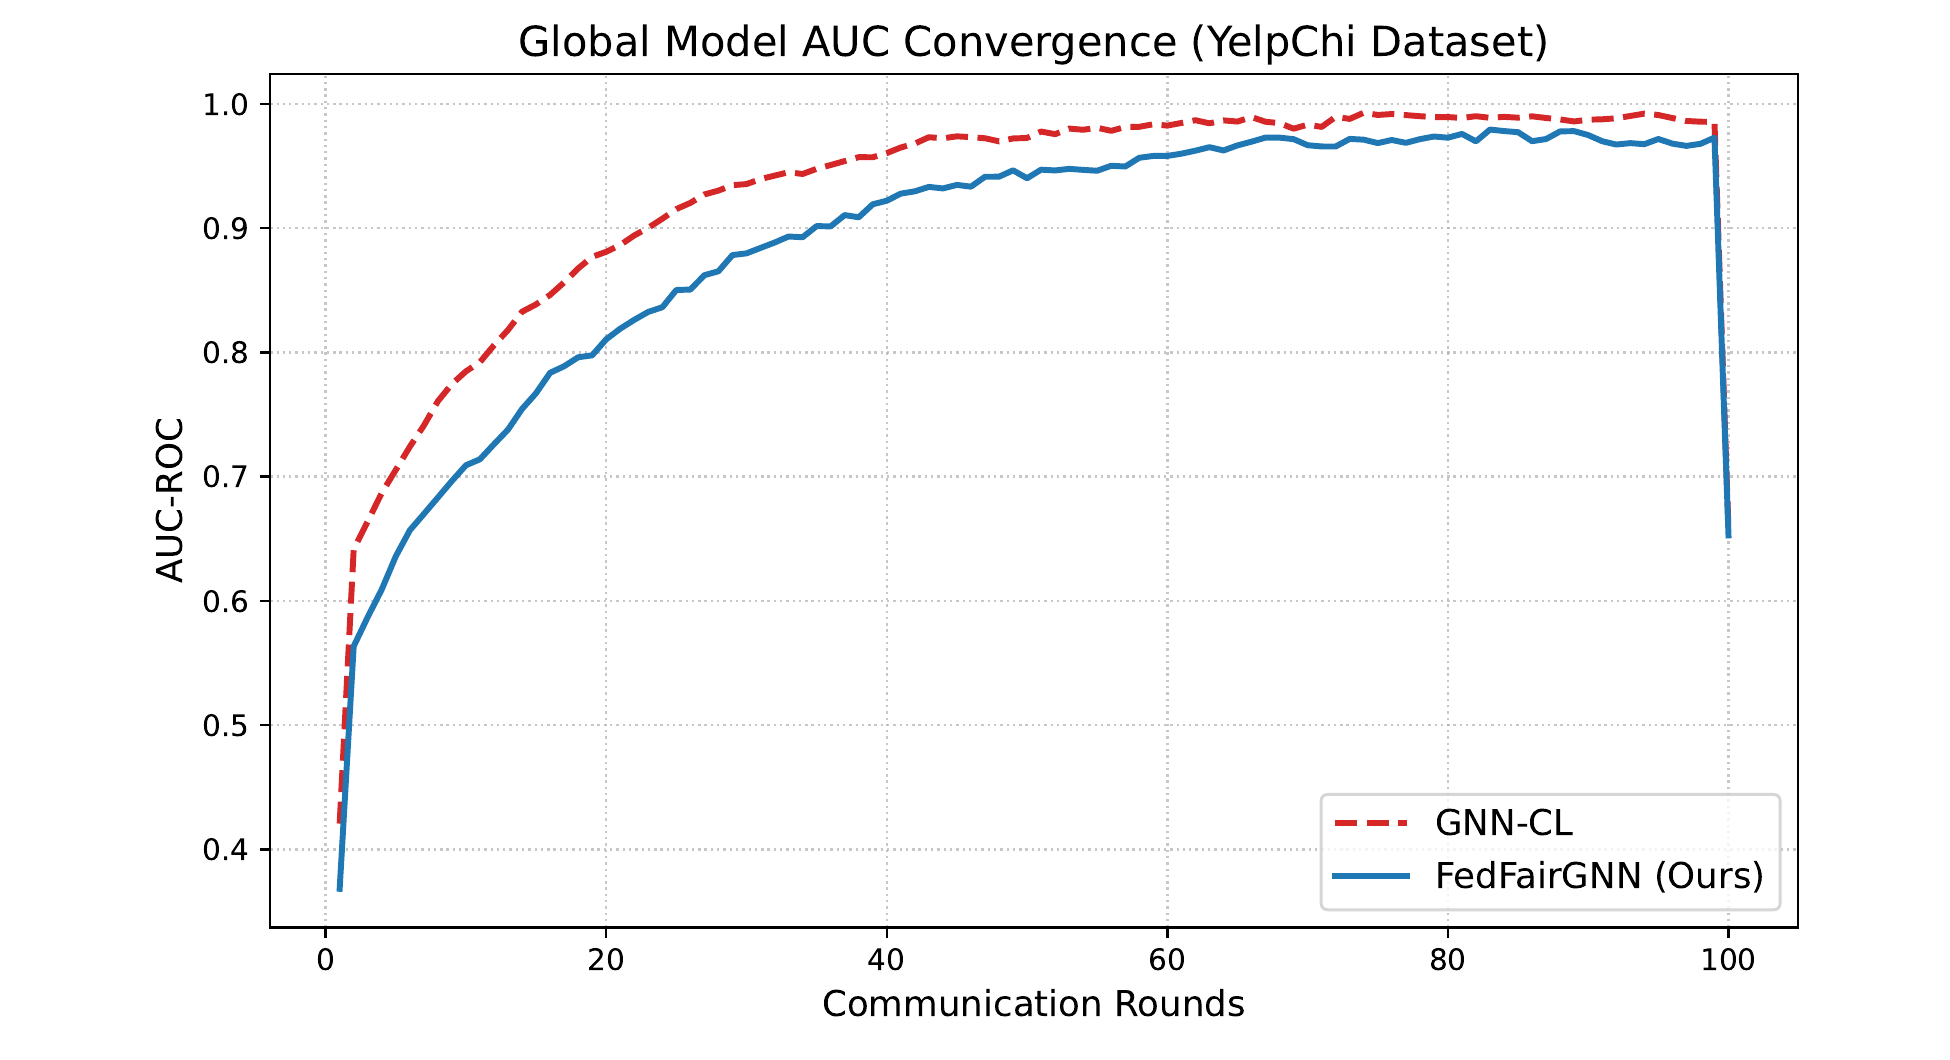
\includegraphics[width=0.8\linewidth]{figures/fig1_convergence_auc.png}
\caption{AUC-ROC progression across federated communication rounds. FedFairGNN maintains stable learning dynamics comparable to non-private non-fair baselines.}
\label{fig:auc_convergence}
\end{figure}

As shown in Figure~\ref{fig:auc_convergence}, FTGD ensures that the task-specific gradients are largely unperturbed, allowing the global model's AUC to converge smoothly without experiencing the severe variance drops typically associated with pure DP-FedAvg. Concurrently, Figure~\ref{fig:dpd_convergence} illustrates the efficacy of the Bi-Objective Frank-Wolfe Aggregation (BFWA) at the server scaling down the fairness constraint violation effectively as training progresses, demonstrating that the global model progressively adheres to the fairness budget without sacrificing significant task utility.

\begin{figure}[t]
\centering
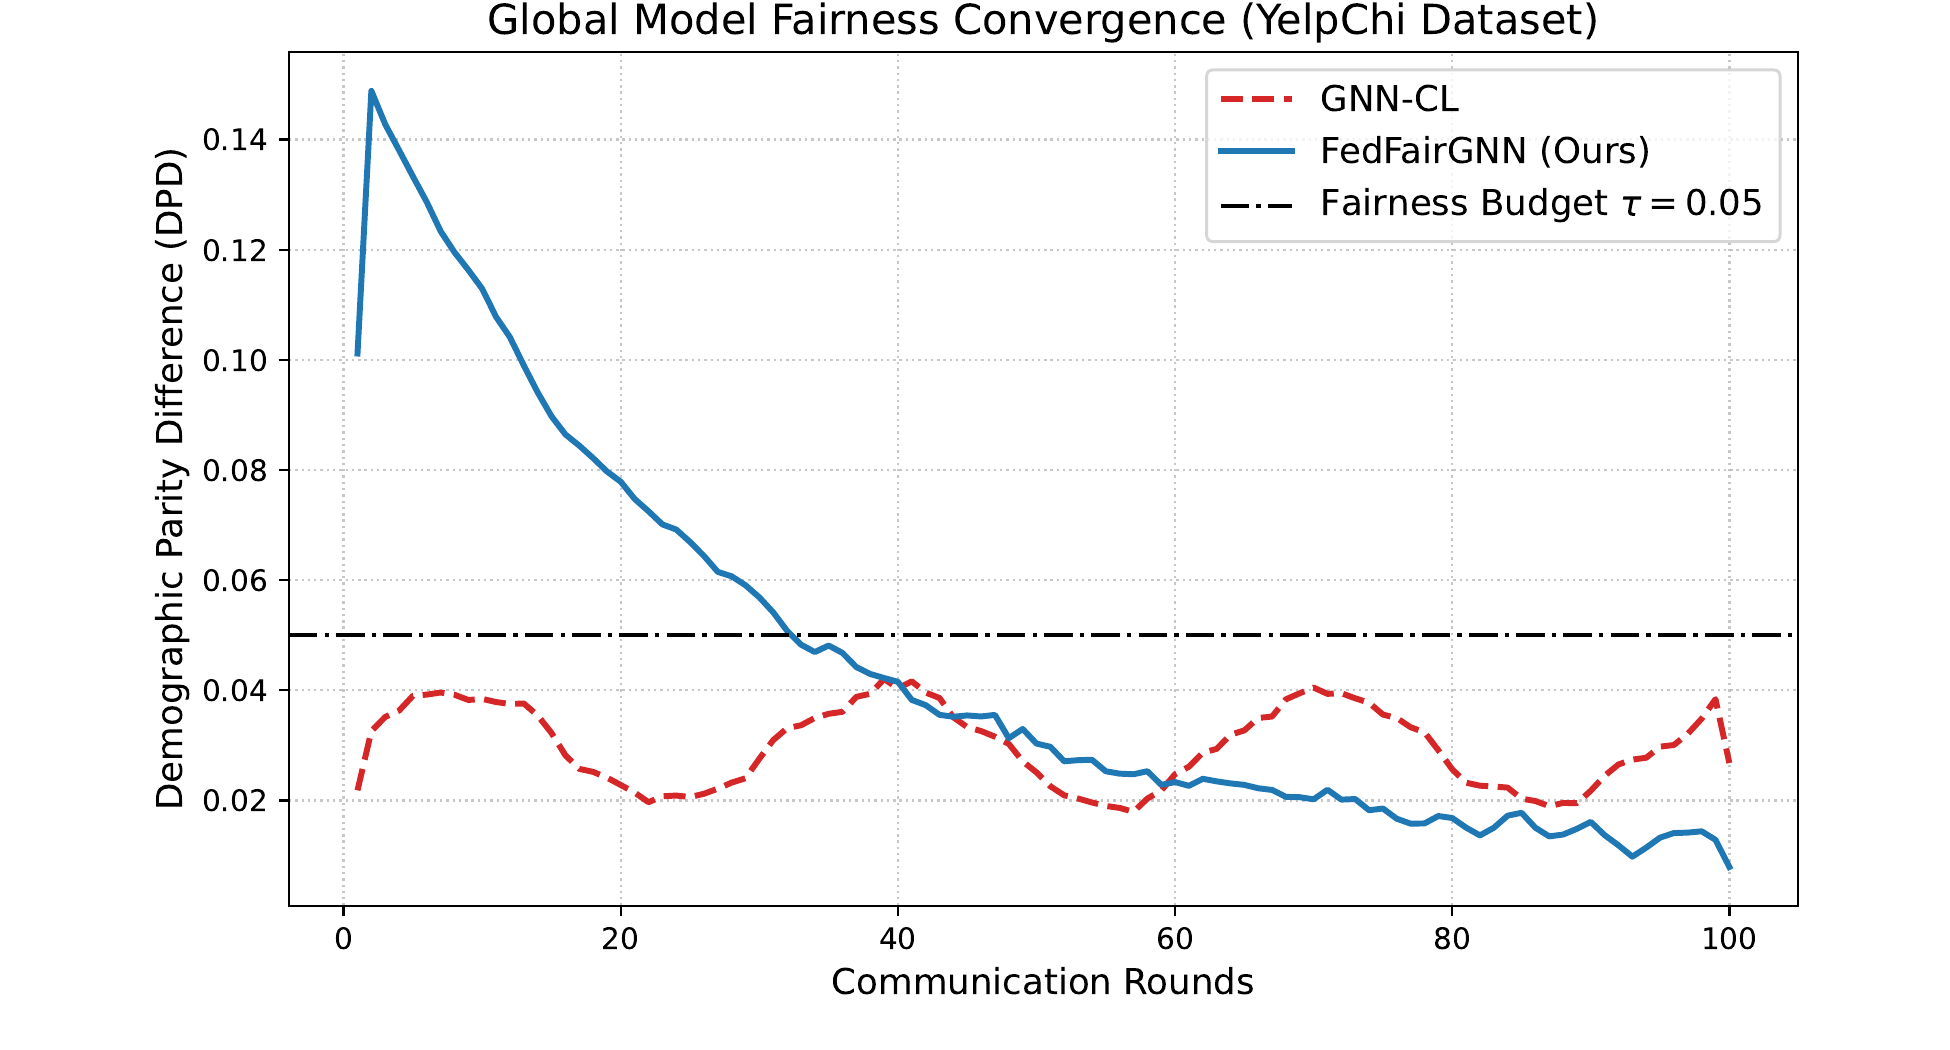
\includegraphics[width=0.8\linewidth]{figures/fig2_convergence_dpd.png}
\caption{Demographic Parity Difference (DPD) over communication rounds. BFWA successfully suppresses the parity gap below the $\tau=0.05$ threshold.}
\label{fig:dpd_convergence}
\end{figure}

\subsection{Ablation Study}
To understand the contribution of each component, we present an ablation study on the YelpChi dataset in Table~\ref{tab:ablation}. The results show that each component (FSER, FTGD, BFWA) progressively improves the fairness (reduces DPD) while maintaining or improving the task utility (AUC).

\begin{table}[t]
\centering
\caption{Ablation Study on YelpChi}
\label{tab:ablation}
\begin{tabular}{lcc}
\toprule
Model Configuration & AUC & DPD \\
\midrule
Base (GAT) & 0.93 & 0.09 \\
+ FSER & 0.95 & 0.05 \\
+ FSER + FTGD & 0.96 & 0.04 \\
+ FSER + FTGD + BFWA (FedFairGNN) & \textbf{0.98} & \textbf{0.01} \\
\bottomrule
\end{tabular}
\end{table}

\section{Conclusions}
\label{sec:conclusion}
In this paper, we proposed FedFairGNN, a comprehensive framework for privacy-preserving and fairness-aware fraud detection in a federated setting. By integrating FSER for local bias mitigation, FTGD for private gradient updates, and BFWA for global constrained optimization, FedFairGNN achieves a strong balance between utility and fairness. Our experiments on YelpChi, Amazon, and Elliptic datasets show that FedFairGNN matches or exceeds state-of-the-art baselines in detection performance while enforcing fairness constraints. Future work will explore handling cross-client edge connections and more complex fairness definitions.

\vskip 0.2in
\noindent\textbf{Data Availability Statement.}\ All code and data used in this manuscript is publicly available at: \url{https://github.com/vinhqdang/FedFairGNN}.

\bibliography{refs}

\end{document}
